% Punto 2 -- Relaciones entre series y modelos estadisticos (Rol B)
% Compilar desde documentos/ con: latexmk -pdf -interaction=nonstopmode -halt-on-error punto2_modelador_rol_b.tex
% Bibliografia: biblatex-apa / Biber, con DOI comprobados contra Crossref y fichas NASA.
\documentclass[12pt,letterpaper]{article}
\usepackage[utf8]{inputenc}
\usepackage[T1]{fontenc}
\usepackage[spanish,es-nodecimaldot,es-noshorthands]{babel}
\usepackage{newtxtext,newtxmath}
\usepackage[margin=2.54cm,headheight=14pt]{geometry}
\usepackage{amsmath,amssymb}
\usepackage{graphicx}
\usepackage{booktabs}
\usepackage{tabularx}
\usepackage{longtable}
\usepackage{array}
\usepackage{float}
\usepackage{caption}
\usepackage{setspace}
\usepackage{fancyhdr}
\usepackage{csquotes}
\usepackage[backend=biber,style=apa,sorting=nyt,sortcites=true]{biblatex}
\DeclareLanguageMapping{spanish}{spanish-apa}
\addbibresource{referencias_punto2_rol_b.bib}
\usepackage{xurl}
\usepackage[hidelinks]{hyperref}

\graphicspath{{../figuras/}}
\captionsetup{font=small,labelfont=bf}
\setlength{\parindent}{1.27cm}
\setlength{\parskip}{0pt}
\setlength{\bibitemsep}{\baselineskip}
\doublespacing
\pagestyle{fancy}
\fancyhf{}
\fancyhead[R]{\thepage}
\renewcommand{\headrulewidth}{0pt}

\newcommand{\apafigureheading}[2]{%
  \refstepcounter{figure}\label{#1}%
  \noindent\textbf{Figura \thefigure}\par
  \noindent\textit{#2}\par\smallskip}
\newcommand{\apatableheading}[2]{%
  \refstepcounter{table}\label{#1}%
  \noindent\textbf{Tabla \thetable}\par
  \noindent\textit{#2}\par\smallskip}
\newcommand{\apanote}[1]{\par\smallskip\noindent{\footnotesize\textit{Nota.} #1}}
\newcommand{\monthname}[1]{%
  \ifcase#1\or Enero\or Febrero\or Marzo\or Abril\or Mayo\or Junio\or Julio\or Agosto\or Septiembre\or Octubre\or Noviembre\or Diciembre\fi}

\title{Punto 2. Relaciones entre series y modelos estadísticos\\
\large Río Maipo en El Manzano (CAMELS-CL 5710001)}
\author{Santiago Ortega\\Rol B -- Modelador\\Tarea 1 de Hidrología\\Universidad Nacional de Colombia}
\date{7 de octubre de 2026}

\begin{document}
\sloppy
\begin{titlepage}
\thispagestyle{fancy}
\centering
\vspace*{2.0cm}
{\bfseries\Large Punto 2. Relaciones entre series y modelos estadísticos\par}
\vspace{0.7cm}
{\large Río Maipo en El Manzano (CAMELS-CL 5710001)\par}
\vspace{1.7cm}
{\large Santiago Ortega\par}
{\normalsize Rol B -- Modelador\par}
\vfill
{\normalsize Tarea 1 de Hidrología\par}
{\normalsize Universidad Nacional de Colombia\par}
{\normalsize 7 de octubre de 2026\par}
\end{titlepage}

\section*{Resumen}
Se compararon las precipitaciones mensuales de referencia e IMERG, y sus relaciones con el caudal medio mensual del Río Maipo en El Manzano. La lluvia local--IMERG presentó correlación alta (Pearson $r=0.888$; Spearman $\rho=0.824$), pero sesgo medio $-5.50$ mm/mes, MAE $27.34$ mm/mes y RMSE $48.66$ mm/mes; los errores variaron con la estación y la intensidad. Las correlaciones contemporáneas lluvia--caudal fueron negativas en las series originales, pero se debilitaron y cambiaron de signo al retirar el ciclo mensual. Los máximos exploratorios de asociación lluvia previa--caudal no se interpretan como tiempos físicos. Se evaluaron correcciones de precipitación y modelos de caudal en tres bloques cronológicos externos no solapados, con selección y climatologías restringidas al ajuste. La corrección de lluvia no superó consistentemente a IMERG sin corregir; el modelo de anomalías con rezago redujo MAE y RMSE del caudal frente a la climatología mensual en los bloques examinados, aunque mantuvo sesgo positivo. La evidencia es retrospectiva y no demuestra causalidad ni estabilidad futura. La versión de los valores IMERG del CSV se identifica como V06 por la configuración vigente y el acuerdo del equipo, pero no se conserva el manifiesto de la exportación original.

\noindent\textit{Palabras clave:} precipitación satelital, anomalías, caudal, validación temporal, Andes centrales.

\section{Contexto, datos y decisiones metodológicas}

\subsection{Fuente, unidades y cobertura}
La fuente única de los cálculos es \texttt{datos/datos\_mensuales\_maipo.csv}. El archivo contiene 484 marcas mensuales entre 1980-01 y 2020-04; \texttt{P\_local\_mm} tiene un faltante en 2020-04 y el caudal tiene 14 faltantes (470 valores válidos, 2.89\%). La precipitación satelital y la temperatura cubren 2000-06--2020-03. Se mantuvieron las series locales completas y se usaron pares completos por pregunta, sin imputar. Las ventanas resultantes son: 238 pares lluvia local--IMERG, 469 pares lluvia local--caudal y 230 pares IMERG--caudal.

Se usaron \texttt{P\_local\_mm} y \texttt{P\_IMERG\_mm} en mm/mes, \texttt{Caudal\_m3s} en m$^3$/s y \texttt{Q\_lamina\_mm} en mm/mes. La lámina se deriva del caudal volumétrico y el área $A=4837.4$ km$^2$:
\begin{equation}
Q_{\mathrm{lamina},m}=\frac{Q_m\,(D_m\,86400)}{A\,10^6}\,1000,
\label{eq:runoff-depth}
\end{equation}
donde $D_m$ es el número de días del mes. Esta conversión cambia unidades, no constituye una fuente independiente de observaciones.

La documentación de CAMELS-CL describe precipitación nacional y global y advierte incertidumbre de precipitación en cabeceras montañosas \parencite{AlvarezGarreton2018}. El script vigente selecciona la colección mensual IMERG V06; la entrada de cierre del equipo adoptó V06 como versión canónica a partir del script y el historial. Sin embargo, la auditoría de procedencia encontró que no se conserva el archivo intermedio, identificador de tarea ni manifiesto del raster que originó el CSV. Por rigor, este informe la denomina \textit{versión documentada/configurada V06}; la trazabilidad de la exportación específica no es completa. NASA define IMERG Final como producto de investigación que incorpora análisis de pluviómetros \parencite{IMERGV06,IMERGV07}.

\subsection{Diseño estadístico}
La regla de pares completos se aplica separadamente a cada relación y se reportan ventana y $n$. En lluvia local--IMERG se definió el error como $e_t=P_{I,t}-P_{L,t}$; por ello, un sesgo negativo indica subestimación promedio de la referencia. Se calcularon sesgo medio, MAE, RMSE y
\begin{equation}
\mathrm{PBIAS}=100\,\frac{\sum_t(P_{I,t}-P_{L,t})}{\sum_t P_{L,t}}.
\end{equation}
Pearson resume asociación lineal y Spearman asociación monótona por rangos; ninguna mide por sí sola concordancia ni demuestra causalidad. MAE conserva la escala del error y RMSE da mayor peso a los errores grandes. Por esa diferencia se interpretan conjuntamente, siguiendo recomendaciones para evaluación de precipitación satelital y modelos hidrológicos \parencite{HossainHuffman2008,Gupta2009,Willmott1981}.

Las anomalías se definieron por mes calendario como $a_{X,t}=X_t-\bar X_{m(t)}$ y las anomalías estandarizadas como $z_{X,t}=a_{X,t}/s_{m(t)}$, con desviación estándar muestral ($ddof=1$). La referencia común fija es 2000-06--2020-03; no hubo desviaciones mensuales nulas. Estandarizar no implica normalidad ni equivale a un índice de sequía. El rezago se define como precipitación en $t-k$ frente a caudal en $t$, sin usar precipitación futura. El barrido de varios rezagos sobre una serie autocorrelacionada se interpreta como exploratorio; la autocorrelación afecta la inferencia de correlaciones \parencite{PyperPeterman1998}.

\section{2.1. Diagramas de dispersión e interpretación}

\subsection{Concordancia entre IMERG y precipitación local}
En los 238 pares de 2000-06 a 2020-03, la correlación fue $r=0.8875$ y $\rho=0.8245$. El sesgo medio $P_I-P_L$ fue $-5.503$ mm/mes, MAE $27.344$ mm/mes, RMSE $48.656$ mm/mes y PBIAS $-8.764\%$. El signo medio no describe cada mes: IMERG estuvo por debajo de la referencia en 103 pares y por encima en 135, y la mediana del error fue $+3.856$ mm/mes. Correlación alta coexiste así con errores relevantes en magnitud.

\begin{table}[H]
\centering\small\singlespacing
\apatableheading{tab:pairmetrics}{Tamaño de muestra y asociación entre series mensuales}
\begin{tabularx}{\textwidth}{lXrrr}
\toprule
Variables & Periodo & $n$ & Pearson $r$ & Spearman $\rho$ \\
\midrule
$P_I$--$P_L$ & 2000-06--2020-03 & 238 & 0.8875 & 0.8245 \\
$P_L$--$Q$ & 1980-01--2020-03 & 469 & $-0.2009$ & $-0.3931$ \\
$P_I$--$Q$ & 2000-06--2020-03 & 230 & $-0.2772$ & $-0.4234$ \\
$P_L$--$R$ & 1980-01--2020-03 & 469 & $-0.1968$ & $-0.3875$ \\
$P_I$--$R$ & 2000-06--2020-03 & 230 & $-0.2708$ & $-0.4145$ \\
\bottomrule
\end{tabularx}
\apanote{Casos completos por par; $P_L$ es la precipitación de referencia, $P_I$ IMERG, $Q$ caudal volumétrico y $R$ lámina equivalente. Fuente: \texttt{figuras/tabla\_2\_1\_metricas\_relaciones.csv}.}
\end{table}

\begin{table}[H]
\centering\small\singlespacing
\apatableheading{tab:rainagreement}{Métricas de error de IMERG respecto de la precipitación local}
\begin{tabular}{lrrrr}
\toprule
Sesgo $P_I-P_L$ (mm/mes) & MAE (mm/mes) & RMSE (mm/mes) & PBIAS (\%) & Mediana del error (mm/mes) \\
\midrule
$-5.503$ & 27.344 & 48.656 & $-8.764$ & $+3.856$ \\
\bottomrule
\end{tabular}
\apanote{PBIAS $=100\sum(P_I-P_L)/\sum P_L$. Sesgo negativo indica que el promedio de IMERG es menor, no que todos los meses sean subestimados.}
\end{table}

\begin{figure}[H]
\centering
\apafigureheading{fig:scatter}{Relaciones mensuales entre precipitación de referencia, IMERG y respuesta de la cuenca}
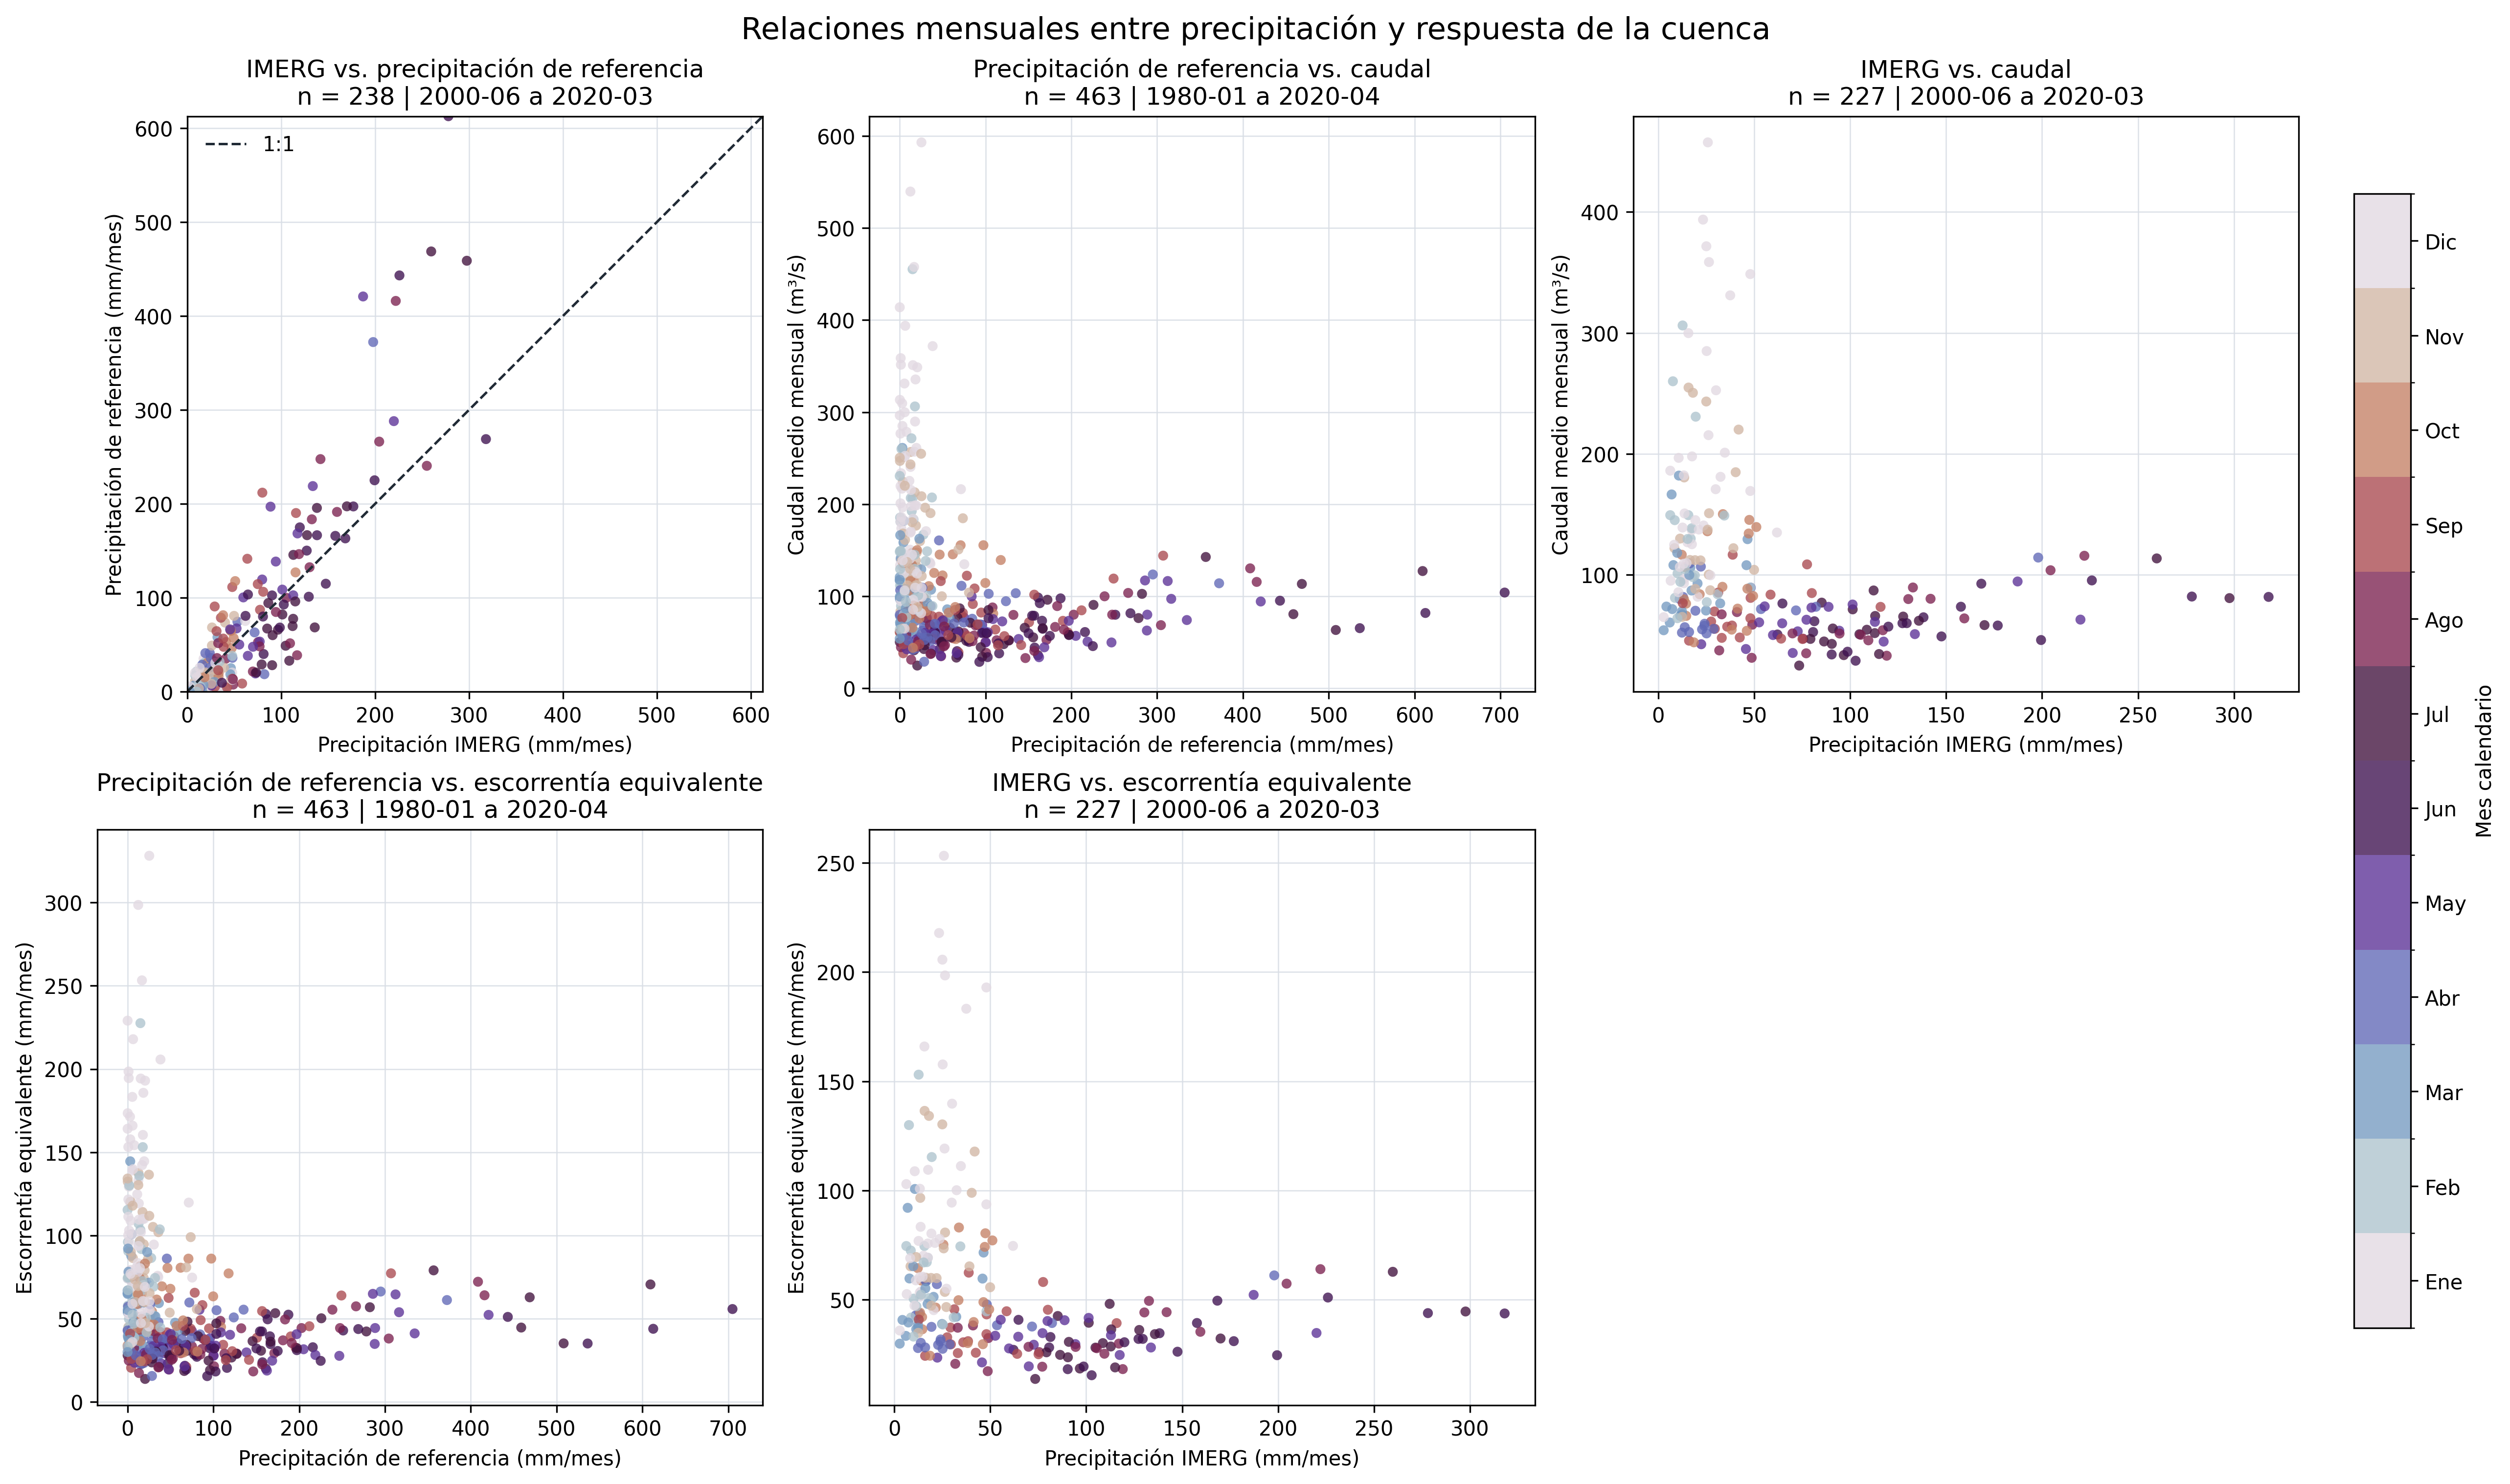
\includegraphics[width=\textwidth]{figura_2_1_relaciones_scatter.png}
\apanote{El panel $P_I$--$P_L$ incluye línea 1:1 y ejes comparables. Los puntos se colorean por mes calendario. Las ventanas y tamaños de muestra se indican en cada panel; $R$ acompaña la relación lluvia--caudal para comparar láminas.}
\end{figure}

La dispersión de $P_I$--$P_L$ se amplía en meses lluviosos. Por estación austral, el sesgo medio fue $+6.85$ mm/mes en verano, $-9.38$ en otoño, $-11.33$ en invierno y $-8.28$ en primavera. Por cuartil de precipitación local, los tres cuartiles inferiores mostraron sesgos positivos (+14.00, +9.97 y +6.43 mm/mes), mientras el cuartil superior mostró $-51.94$ mm/mes y RMSE de 88.52 mm/mes. La literatura demuestra que el error de IMERG puede depender de intensidad y densidad de pluviómetros en otros dominios; esos mecanismos motivan el desglose, pero no transfieren sus magnitudes a Maipo \parencite{Tian2018,HosseiniMoghari2020}.

\begin{table}[H]
\centering\small\singlespacing
\apatableheading{tab:groupErrors}{Error de IMERG por estación austral e intensidad de precipitación local}
\begin{tabularx}{\textwidth}{llrrrr}
\toprule
Agrupación & Clase & $n$ & Sesgo $P_I-P_L$ & MAE & RMSE \\
 & & & \multicolumn{3}{c}{mm/mes} \\
\midrule
Estación & Verano & 60 & $+6.85$ & 11.26 & 14.20 \\
 & Otoño & 58 & $-9.38$ & 26.12 & 47.76 \\
 & Invierno & 60 & $-11.33$ & 49.10 & 76.72 \\
 & Primavera & 60 & $-8.28$ & 22.85 & 33.13 \\
Cuartil $P_L$ & Q1 (0--8.53] & 60 & $+14.00$ & 14.09 & 17.06 \\
 & Q2 (8.53--25.56] & 59 & $+9.97$ & 13.49 & 20.54 \\
 & Q3 (25.56--78.47] & 59 & $+6.43$ & 22.74 & 29.39 \\
 & Q4 (78.47--612.67] & 60 & $-51.94$ & 58.75 & 88.52 \\
\bottomrule
\end{tabularx}
\apanote{Los cuartiles se definieron con $P_L$ de los 238 pares. No se excluyeron eventos extremos del resultado principal. Fuente: \texttt{figuras/tabla\_2\_1\_errores\_por\_grupo.csv}.}
\end{table}

Los cinco errores absolutos mayores suman 52.35\% del error cuadrático total. Son episodios para verificar frente a las fuentes originales, no datos que deban eliminarse automáticamente.

\begin{table}[H]
\centering\small\singlespacing
\apatableheading{tab:influential}{Cinco meses con mayor error absoluto $P_I-P_L$}
\begin{tabular}{lrrrr}
\toprule
Mes & $P_L$ (mm/mes) & $P_I$ (mm/mes) & Error (mm/mes) & Estación \\
\midrule
2000-06 & 612.67 & 278.06 & $-334.60$ & Invierno \\
2008-05 & 420.78 & 187.26 & $-233.52$ & Otoño \\
2005-06 & 443.17 & 225.96 & $-217.22$ & Invierno \\
2006-07 & 468.70 & 259.77 & $-208.93$ & Invierno \\
2005-08 & 416.03 & 222.05 & $-193.99$ & Invierno \\
\bottomrule
\end{tabular}
\apanote{Sensibilidad descriptiva al excluir estos cinco meses: Pearson cambia de 0.8875 a 0.8829 y RMSE de 48.66 a 33.94 mm/mes. La serie principal los conserva.}
\end{table}

\subsection{Relación contemporánea y respuesta estacional}
En las series originales, las correlaciones contemporáneas lluvia--caudal son negativas. Al quitar la media mensual, la asociación contemporánea se vuelve débilmente positiva: $r=0.1569$ para lluvia local--Q y $r=0.1783$ para IMERG--Q. El cambio evidencia que el ciclo anual compartido influye en la correlación original. No se interpreta como contradicción: son preguntas estadísticas distintas, asociación entre niveles mensuales frente a covariación de anomalías.

\begin{table}[H]
\centering\small\singlespacing
\apatableheading{tab:monthlyCycle}{Medias climatológicas mensuales en la referencia común 2000-06--2020-03}
\begin{tabular}{lrrrrr}
\toprule
Mes & $n_{P_L}$ & $P_L$ (mm/mes) & $P_I$ (mm/mes) & $n_Q$ & $Q$ (m$^3$/s) \\
\midrule
Enero & 20 & 13.41 & 18.02 & 20 & 177.99 \\
Febrero & 20 & 12.28 & 17.49 & 20 & 133.96 \\
Marzo & 20 & 10.75 & 17.07 & 20 & 93.39 \\
Abril & 19 & 44.40 & 37.48 & 18 & 72.55 \\
Mayo & 19 & 116.87 & 88.51 & 18 & 59.15 \\
Junio & 20 & 168.08 & 140.24 & 19 & 60.98 \\
Julio & 20 & 123.72 & 124.97 & 19 & 58.92 \\
Agosto & 20 & 118.27 & 110.88 & 19 & 61.22 \\
Septiembre & 20 & 68.98 & 49.16 & 19 & 68.88 \\
Octubre & 20 & 39.75 & 35.26 & 19 & 95.43 \\
Noviembre & 20 & 24.92 & 24.38 & 19 & 146.08 \\
Diciembre & 20 & 13.83 & 24.55 & 20 & 192.03 \\
\bottomrule
\end{tabular}
\apanote{Las climatologías mensuales no son intervalos de confianza. La precipitación de referencia e IMERG comparten las mismas fechas válidas en esta ventana. Fuente: \texttt{figuras/tabla\_2\_2\_climatologia\_referencia.csv}.}
\end{table}

La climatología presenta máximos de lluvia en junio y de caudal en diciembre, con unos seis meses de separación. Estudios en Andes centrales y cuencas chilenas documentan la relevancia de nieve, almacenamiento subterráneo y glaciares para la respuesta cálida; Ayala et al. estudiaron específicamente el escurrimiento glaciar del Maipo. La compatibilidad física apoya una hipótesis de almacenamiento, no prueba que ese mecanismo cause por sí solo los rezagos observados \parencite{Masiokas2006,Cortes2017,AlvarezGarreton2021,Ayala2020}.

\subsection{Anomalías y rezagos exploratorios}
El máximo de Pearson local ocurrió en $k=7$ meses ($r=0.4773$, $n=463$); para IMERG también en $k=7$ ($r=0.4222$, $n=224$). Los valores exploratorios dependen de la climatología y del conjunto de pares; se evaluaron 13 rezagos sobre series autocorrelacionadas. El máximo seleccionado de una exploración no equivale a un tiempo físico de deshielo ni a una significancia inferencial; los problemas de dependencia temporal en las correlaciones están documentados \parencite{PyperPeterman1998}.

\begin{figure}[H]
\centering
\apafigureheading{fig:lags}{Correlación entre precipitación antecedente y caudal actual en anomalías mensuales}
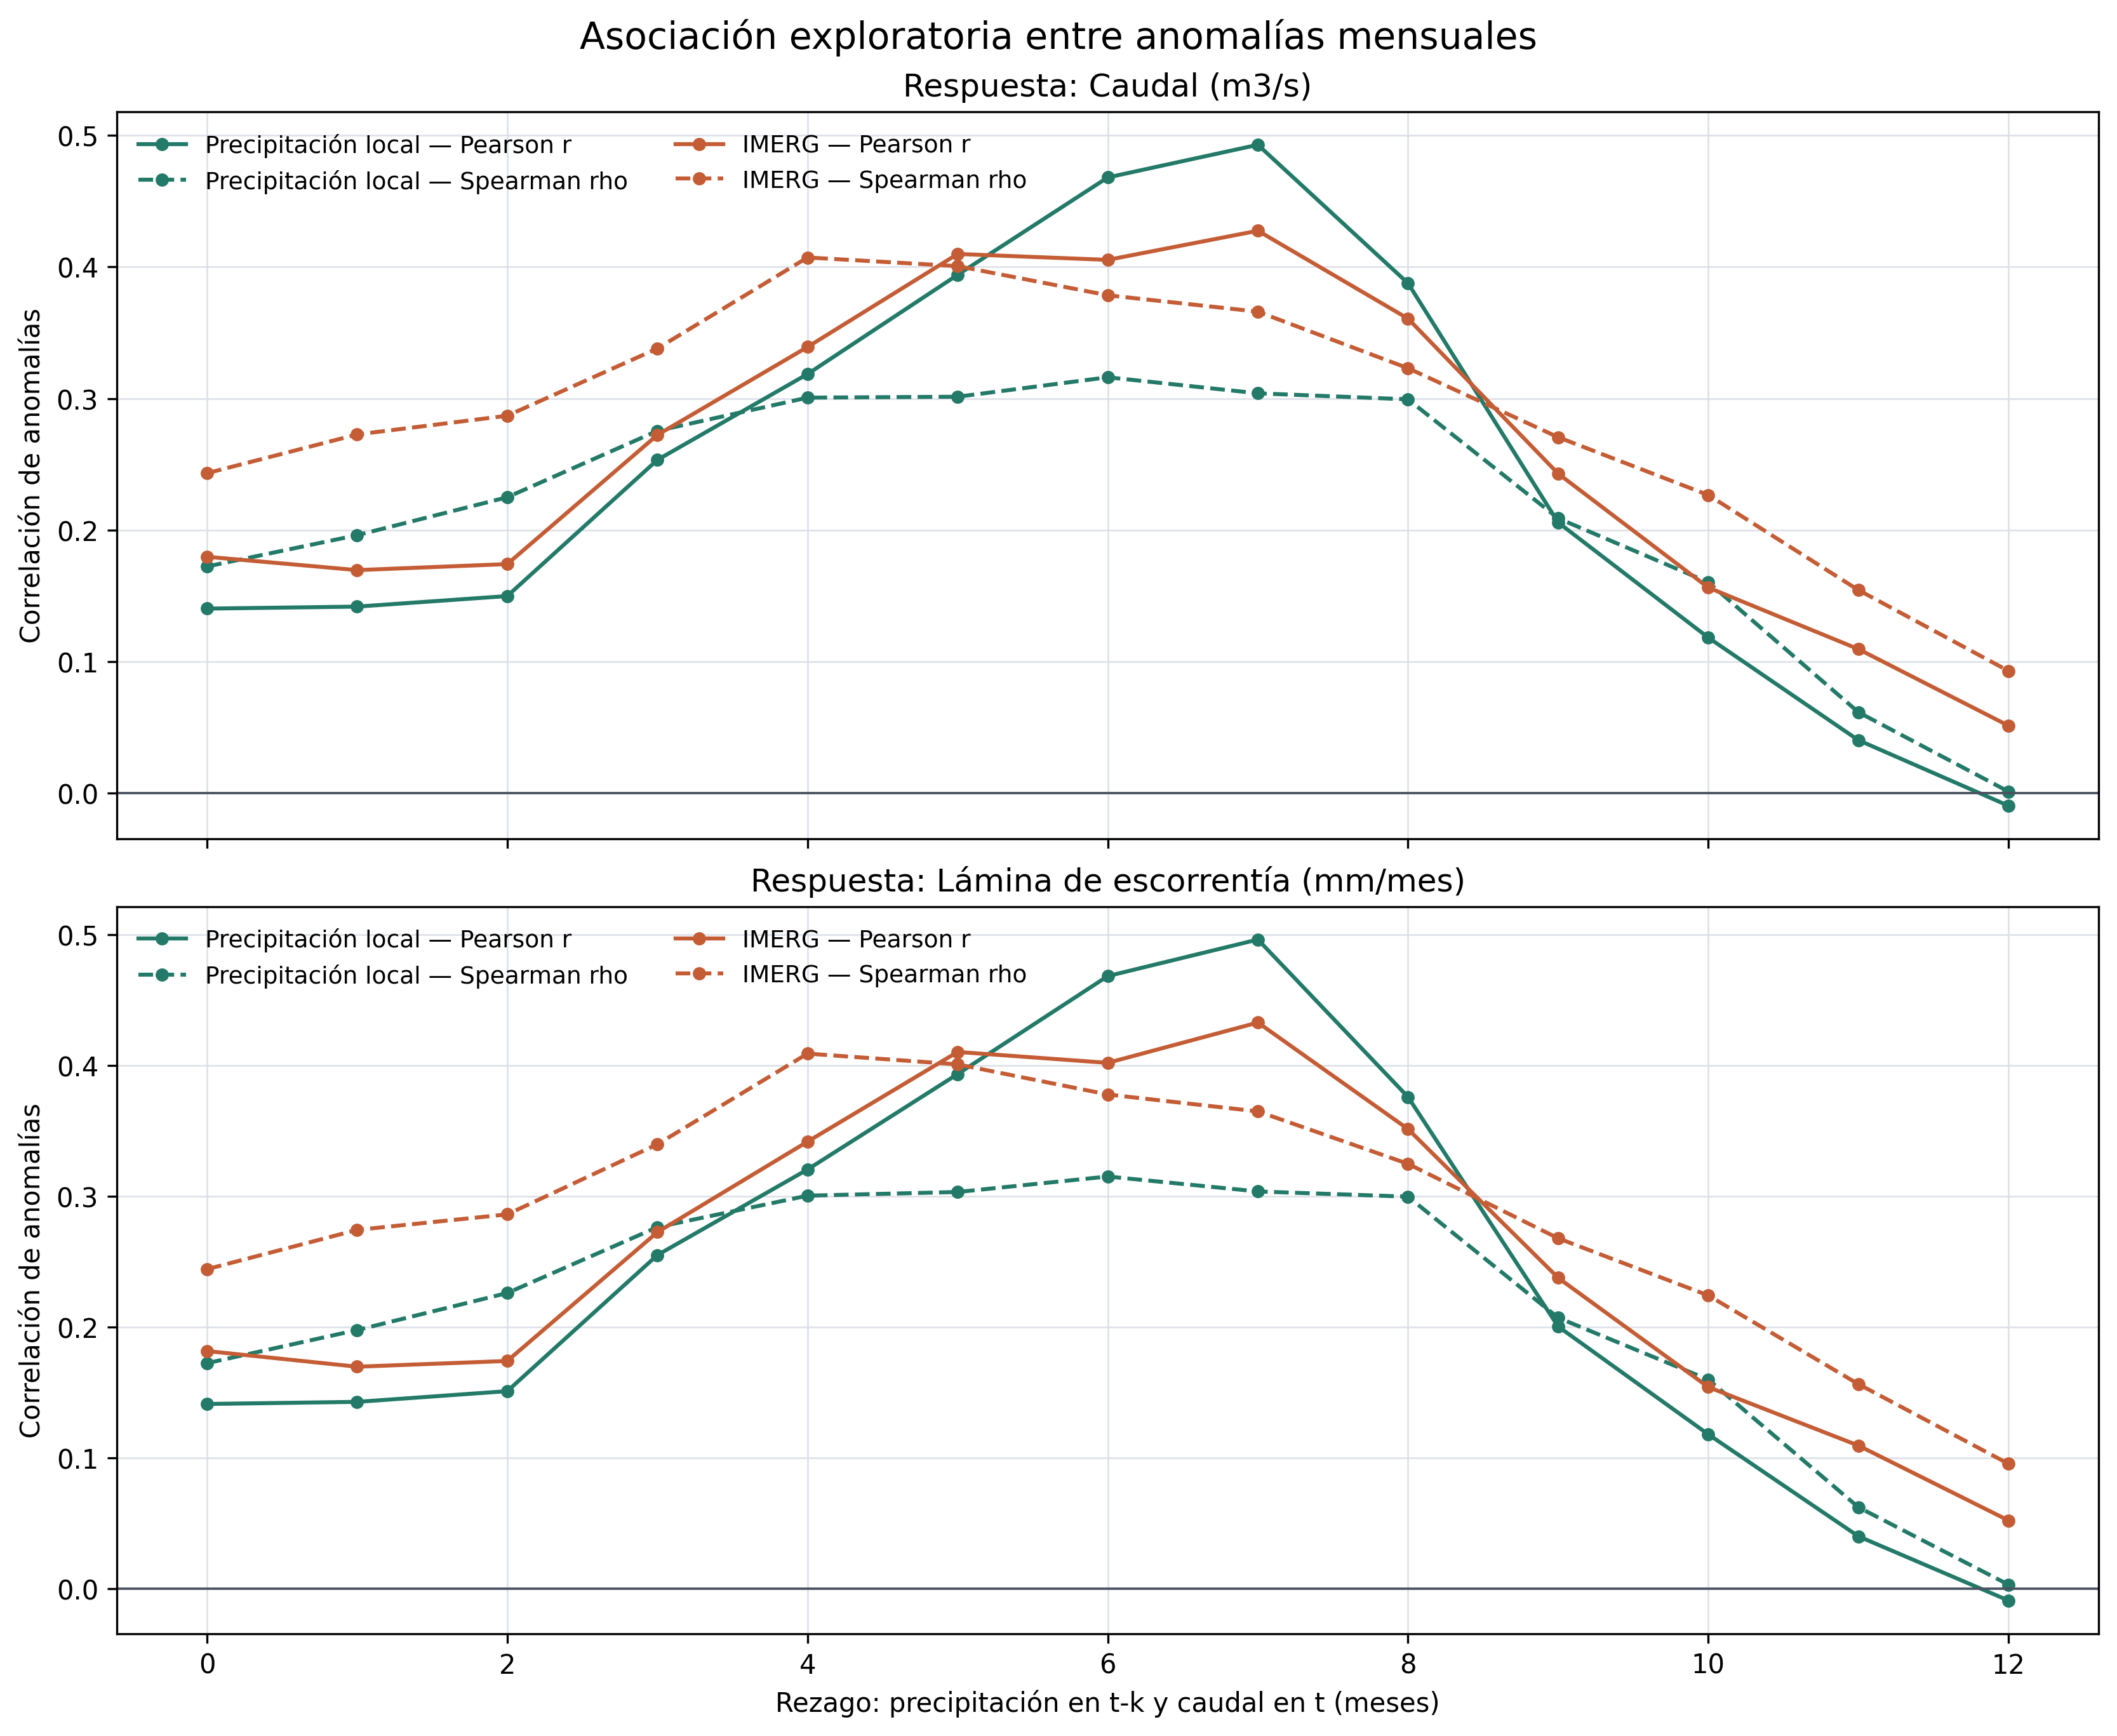
\includegraphics[width=\textwidth]{figura_2_2_correlaciones_rezagos.png}
\apanote{Rezago $k$: precipitación en $t-k$ frente a caudal en $t$. Curvas muestran Pearson y Spearman para lluvia local e IMERG. Análisis exploratorio sin intervalos de incertidumbre ajustados por dependencia/múltiples lags.}
\end{figure}

\begin{table}[H]
\centering\footnotesize\singlespacing
\apatableheading{tab:lagCorrelations}{Correlaciones de anomalías por rezago de precipitación}
\begin{tabular}{rrrrrrrr}
\toprule
$k$ & $n_L$ & $r_L$ & $\rho_L$ & $n_I$ & $r_I$ & $\rho_I$ & Sentido \\
\midrule
0 & 469 & .157 & .175 & 230 & .178 & .237 & $P(t)$--$Q(t)$ \\
1 & 469 & .152 & .207 & 230 & .168 & .269 & $P(t-1)$--$Q(t)$ \\
2 & 468 & .146 & .229 & 229 & .175 & .295 & $P(t-2)$--$Q(t)$ \\
3 & 467 & .253 & .279 & 228 & .273 & .344 & $P(t-3)$--$Q(t)$ \\
4 & 466 & .315 & .305 & 227 & .332 & .410 & $P(t-4)$--$Q(t)$ \\
5 & 465 & .380 & .291 & 226 & .409 & .398 & $P(t-5)$--$Q(t)$ \\
6 & 464 & .454 & .304 & 225 & .393 & .357 & $P(t-6)$--$Q(t)$ \\
7 & 463 & .477 & .295 & 224 & .422 & .355 & $P(t-7)$--$Q(t)$ \\
8 & 462 & .380 & .304 & 223 & .359 & .319 & $P(t-8)$--$Q(t)$ \\
9 & 461 & .195 & .208 & 222 & .241 & .266 & $P(t-9)$--$Q(t)$ \\
10 & 460 & .100 & .148 & 221 & .157 & .232 & $P(t-10)$--$Q(t)$ \\
11 & 459 & .047 & .067 & 220 & .109 & .151 & $P(t-11)$--$Q(t)$ \\
12 & 458 & .005 & .004 & 219 & .051 & .092 & $P(t-12)$--$Q(t)$ \\
\bottomrule
\end{tabular}
\apanote{Subíndices $L$ e $I$ denotan precipitaciones local e IMERG. Ventana completa válida por rezago; las muestras cambian al desplazar las series. Fuente: \texttt{figuras/tabla\_2\_2\_correlaciones\_rezagos.csv}.}
\end{table}

\section{2.2. Modelos para lluvia local y caudal}

\subsection{Modelos candidatos y ecuaciones}
Se comparó la referencia sin corregir con regresiones de corrección de lluvia, y para caudal con una climatología mensual, regresión contemporánea y regresión de anomalías con rezago. La selección de modelo/rezago se hizo exclusivamente en una ventana interna de tres años, anterior al bloque externo. En cada partición se reajustaron parámetros con todo el entrenamiento disponible antes del test.

Para estimar lluvia local desde IMERG se consideró la corrección lineal
\begin{equation}
\widehat{P}_{L,t}=\max(0,\beta_{0,b}+\beta_{1,b}P_{I,t}),
\label{eq:rain-linear}
\end{equation}
y una alternativa log-lineal
\begin{equation}
\widehat{P}_{L,t}=\max\!\left(0,S_b\left[\exp\{\gamma_{0,b}+\gamma_{1,b}\ln(1+P_{I,t})\}-1\right]\right),
\label{eq:rain-log}
\end{equation}
donde $S_b$ es el factor de retrans formación por *smearing* estimado en el entrenamiento del bloque $b$. Los valores negativos previos a la truncación inferior se contabilizaron; las predicciones finales negativas fueron cero.

Para caudal, la referencia mensual usa $\bar Q_{m,\mathrm{train}}$ calculada solo con ajuste; la regresión contemporánea usa $\hat Q_t=b_{0,b}+b_{1,b}P_t$. El modelo de anomalías es
\begin{equation}
\widehat{Q}_t=\bar Q_{m(t),\mathrm{train}}+\alpha_b+\beta_b\left[P_{t-k_b}-\bar P_{m(t-k_b),\mathrm{train}}\right],
\label{eq:flow-anomaly}
\end{equation}
con $k_b$ seleccionado en el tuning interno. La estructura es una relación empírica de predicción, no un balance de masa ni un modelo físico completo; no representa explícitamente evapotranspiración, almacenamiento, regulación ni las reservas de nieve/glaciar.

\begin{table}[H]
\centering\footnotesize\singlespacing
\apatableheading{tab:fitVariants}{Transformaciones y coeficientes seleccionados dentro de cada bloque}
\begin{tabularx}{\textwidth}{llXrrrr}
\toprule
Objetivo & Bloque & Modelo/rezago & $\alpha$ & $\beta$ & Intercepto lineal & Pendiente lineal \\
\midrule
$P_L$ & 1 & Lineal corregido & -- & -- & $-22.267$ & 1.520 \\
$P_L$ & 2 & Log-lineal; $S=1.384$ & -- & -- & $-1.394$ & 1.273 \\
$P_L$ & 3 & Lineal corregido & -- & -- & $-18.167$ & 1.411 \\
$Q$ de $P_L$ & 1 & Anomalía, $k=6$ & .010 & .295 & 137.892 & $-.183$ \\
$Q$ de $P_L$ & 2 & Anomalía, $k=7$ & $-.229$ & .336 & 131.819 & $-.171$ \\
$Q$ de $P_L$ & 3 & Anomalía, $k=7$ & $-.079$ & .343 & 128.597 & $-.167$ \\
$Q$ de $P_I$ & 1 & Anomalía, $k=10$ & .923 & .167 & 158.591 & $-.457$ \\
$Q$ de $P_I$ & 2 & Anomalía, $k=7$ & $-6.281$ & .636 & 139.561 & $-.393$ \\
$Q$ de $P_I$ & 3 & Anomalía, $k=7$ & $-9.266$ & .630 & 132.005 & $-.375$ \\
\bottomrule
\end{tabularx}
\apanote{En las filas de caudal, $\alpha$ y $\beta$ son los parámetros del modelo de anomalías; intercepto y pendiente lineal corresponden a $Q\sim P(t)$. En filas de lluvia, intercepto y pendiente son los de la forma seleccionada y reajustada en el ajuste completo del bloque. Unidades: lluvia en mm/mes y caudal en m$^3$/s.}
\end{table}

\subsection{Comparación agregada de los bloques externos}
Los bloques test fueron 2010-01--2012-12, 2013-01--2015-12 y 2016-01--2020-03. Son no solapados; el entrenamiento es expansivo y la muestra de un bloque anterior pasa a estar disponible en el siguiente, por lo que no constituyen réplicas independientes. En la selección de anomalías, la climatología del predictor y del caudal se vuelve a estimar solo en el ajuste de cada fold. Esto reduce fuga temporal, aunque la evaluación sigue siendo retrospectiva.

\begin{table}[H]
\centering\small\singlespacing
\apatableheading{tab:pooledMetrics}{Métricas agregadas sobre predicciones externas de los tres bloques}
\begin{tabularx}{\textwidth}{Xlrrrr}
\toprule
Objetivo / predictor & Modelo & $n$ & Sesgo & MAE & RMSE \\
 & & & \multicolumn{3}{c}{(mm/mes o m$^3$/s)} \\
\midrule
$P_L$ desde $P_I$ & IMERG sin corrección & 123 & 1.239 & 18.411 & 28.050 \\
$P_L$ desde $P_I$ & Corrección seleccionada & 123 & 5.546 & 21.653 & 33.312 \\
$Q$ desde $P_L$ & Climatología mensual $Q$ & 115 & 45.475 & 46.390 & 59.164 \\
$Q$ desde $P_L$ & Regresión lineal $Q\sim P(t)$ & 115 & 46.883 & 54.166 & 59.332 \\
$Q$ desde $P_L$ & Anomalía con rezago & 115 & 37.778 & 39.756 & 50.684 \\
$Q$ desde $P_I$ & Climatología mensual $Q$ & 115 & 45.475 & 46.390 & 59.164 \\
$Q$ desde $P_I$ & Regresión lineal $Q\sim P(t)$ & 115 & 45.931 & 53.150 & 58.443 \\
$Q$ desde $P_I$ & Anomalía con rezago & 115 & 34.507 & 39.600 & 52.746 \\
\bottomrule
\end{tabularx}
\apanote{Sesgo = predicción $-$ observado. Las ventanas agregadas contienen predicciones fuera del ajuste; las climatologías, selección y coeficientes se estimaron por fold. Fuentes: \texttt{figuras/tabla\_2\_3\_metricas\_fuera\_ajuste.csv} y \texttt{figuras/tabla\_2\_3\_predicciones\_fuera\_ajuste.csv}.}
\end{table}

La corrección de $P_I$ no mejora el MAE/RMSE agregado: MAE y RMSE suben respecto de IMERG crudo, aunque la corrección lineal del bloque 3 reduce RMSE dentro de ese bloque. Por ello no se recomienda afirmar que la corrección mejora la lluvia local en general. Para $Q$, el modelo de anomalías con rezago reduce MAE y RMSE frente a la climatología mensual en cada bloque para ambos predictores; conserva sesgo positivo. La regresión contemporánea no mejora uniformemente frente al baseline.

\begin{table}[H]
\centering\footnotesize\singlespacing
\apatableheading{tab:blockMetrics}{MAE/RMSE en cada bloque externo y rezagos seleccionados para caudal}
\begin{tabular}{llrrrrrr}
\toprule
Objetivo & Bloque & $n$ & $k$ & Baseline MAE/RMSE & Lineal MAE/RMSE & Rezago MAE/RMSE & Sesgo rezago \\
\midrule
$P_L$ desde $P_I$ & 1 & 36 & -- & 17.25/23.51 & 21.94/31.79 & -- & -- \\
$P_L$ desde $P_I$ & 2 & 36 & -- & 18.96/25.14 & 22.50/37.97 & -- & -- \\
$P_L$ desde $P_I$ & 3 & 51 & -- & 18.84/32.58 & 20.85/30.74 & -- & -- \\
$Q$ desde $P_L$ & 1 & 36 & 6 & 50.76/64.97 & 60.64/65.37 & 43.21/54.78 & 42.90 \\
$Q$ desde $P_L$ & 2 & 28 & 7 & 48.02/58.47 & 50.60/55.40 & 38.44/48.54 & 36.86 \\
$Q$ desde $P_L$ & 3 & 51 & 7 & 42.41/55.10 & 51.56/56.88 & 38.04/48.80 & 34.67 \\
$Q$ desde $P_I$ & 1 & 36 & 10 & 50.76/64.97 & 65.75/70.44 & 49.25/64.06 & 48.16 \\
$Q$ desde $P_I$ & 2 & 28 & 7 & 48.02/58.47 & 48.06/52.21 & 33.67/45.53 & 31.78 \\
$Q$ desde $P_I$ & 3 & 51 & 7 & 42.41/55.10 & 47.05/51.99 & 36.05/47.32 & 26.37 \\
\bottomrule
\end{tabular}
\apanote{Los valores de cada celda MAE/RMSE están en mm/mes para estimación de lluvia y m$^3$/s para caudal; sesgo del modelo con rezago en m$^3$/s. Bloque 1 = 2010--2012; bloque 2 = 2013--2015; bloque 3 = 2016--2020-03. Fuentes: \texttt{figuras/tabla\_2\_3\_metricas\_por\_bloque.csv} y \texttt{figuras/tabla\_2\_3\_seleccion\_modelos\_ajuste.csv}.}
\end{table}

\begin{figure}[H]
\centering
\apafigureheading{fig:validation}{Predicciones y residuos en los bloques externos}
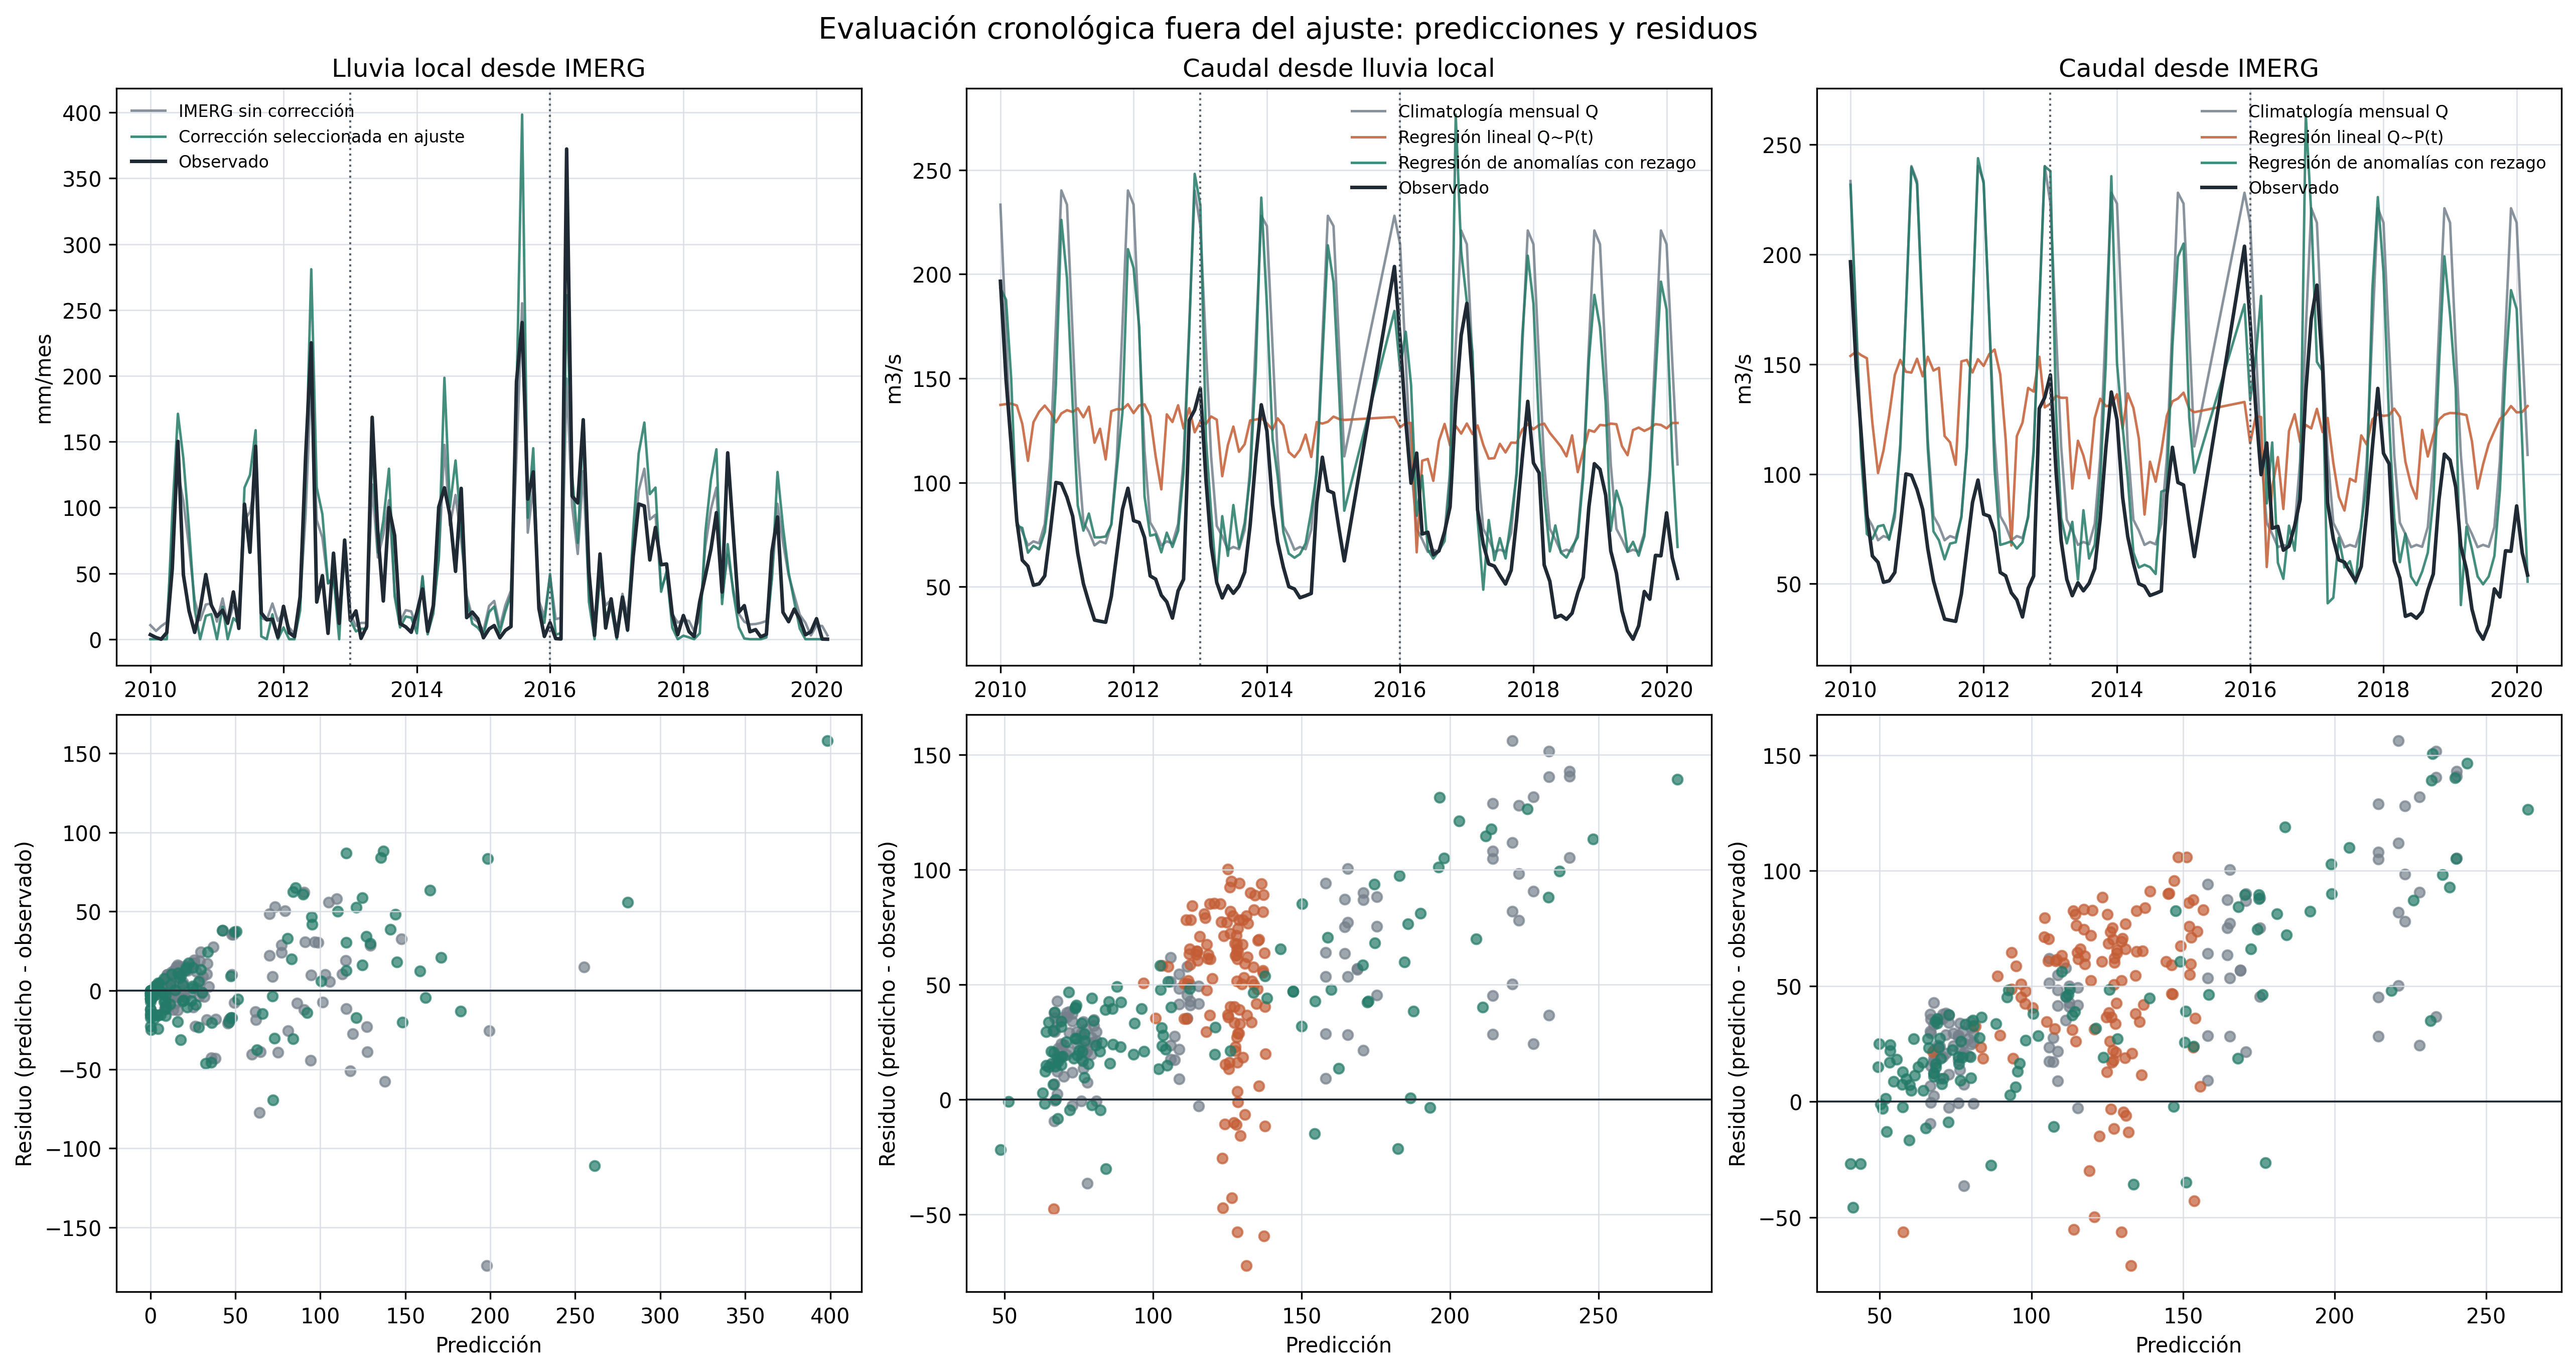
\includegraphics[width=\textwidth]{figura_2_3_validacion_modelos.png}
\apanote{La figura muestra los tres objetivos/modelos sobre sus ventanas de test y los residuos frente al valor predicho. Las líneas verticales marcan cambios de bloque; el diagnóstico visual se complementa con métricas tabuladas, no las sustituye.}
\end{figure}

\begin{figure}[H]
\centering
\apafigureheading{fig:residuals}{Residuos temporales en el test cronológico}
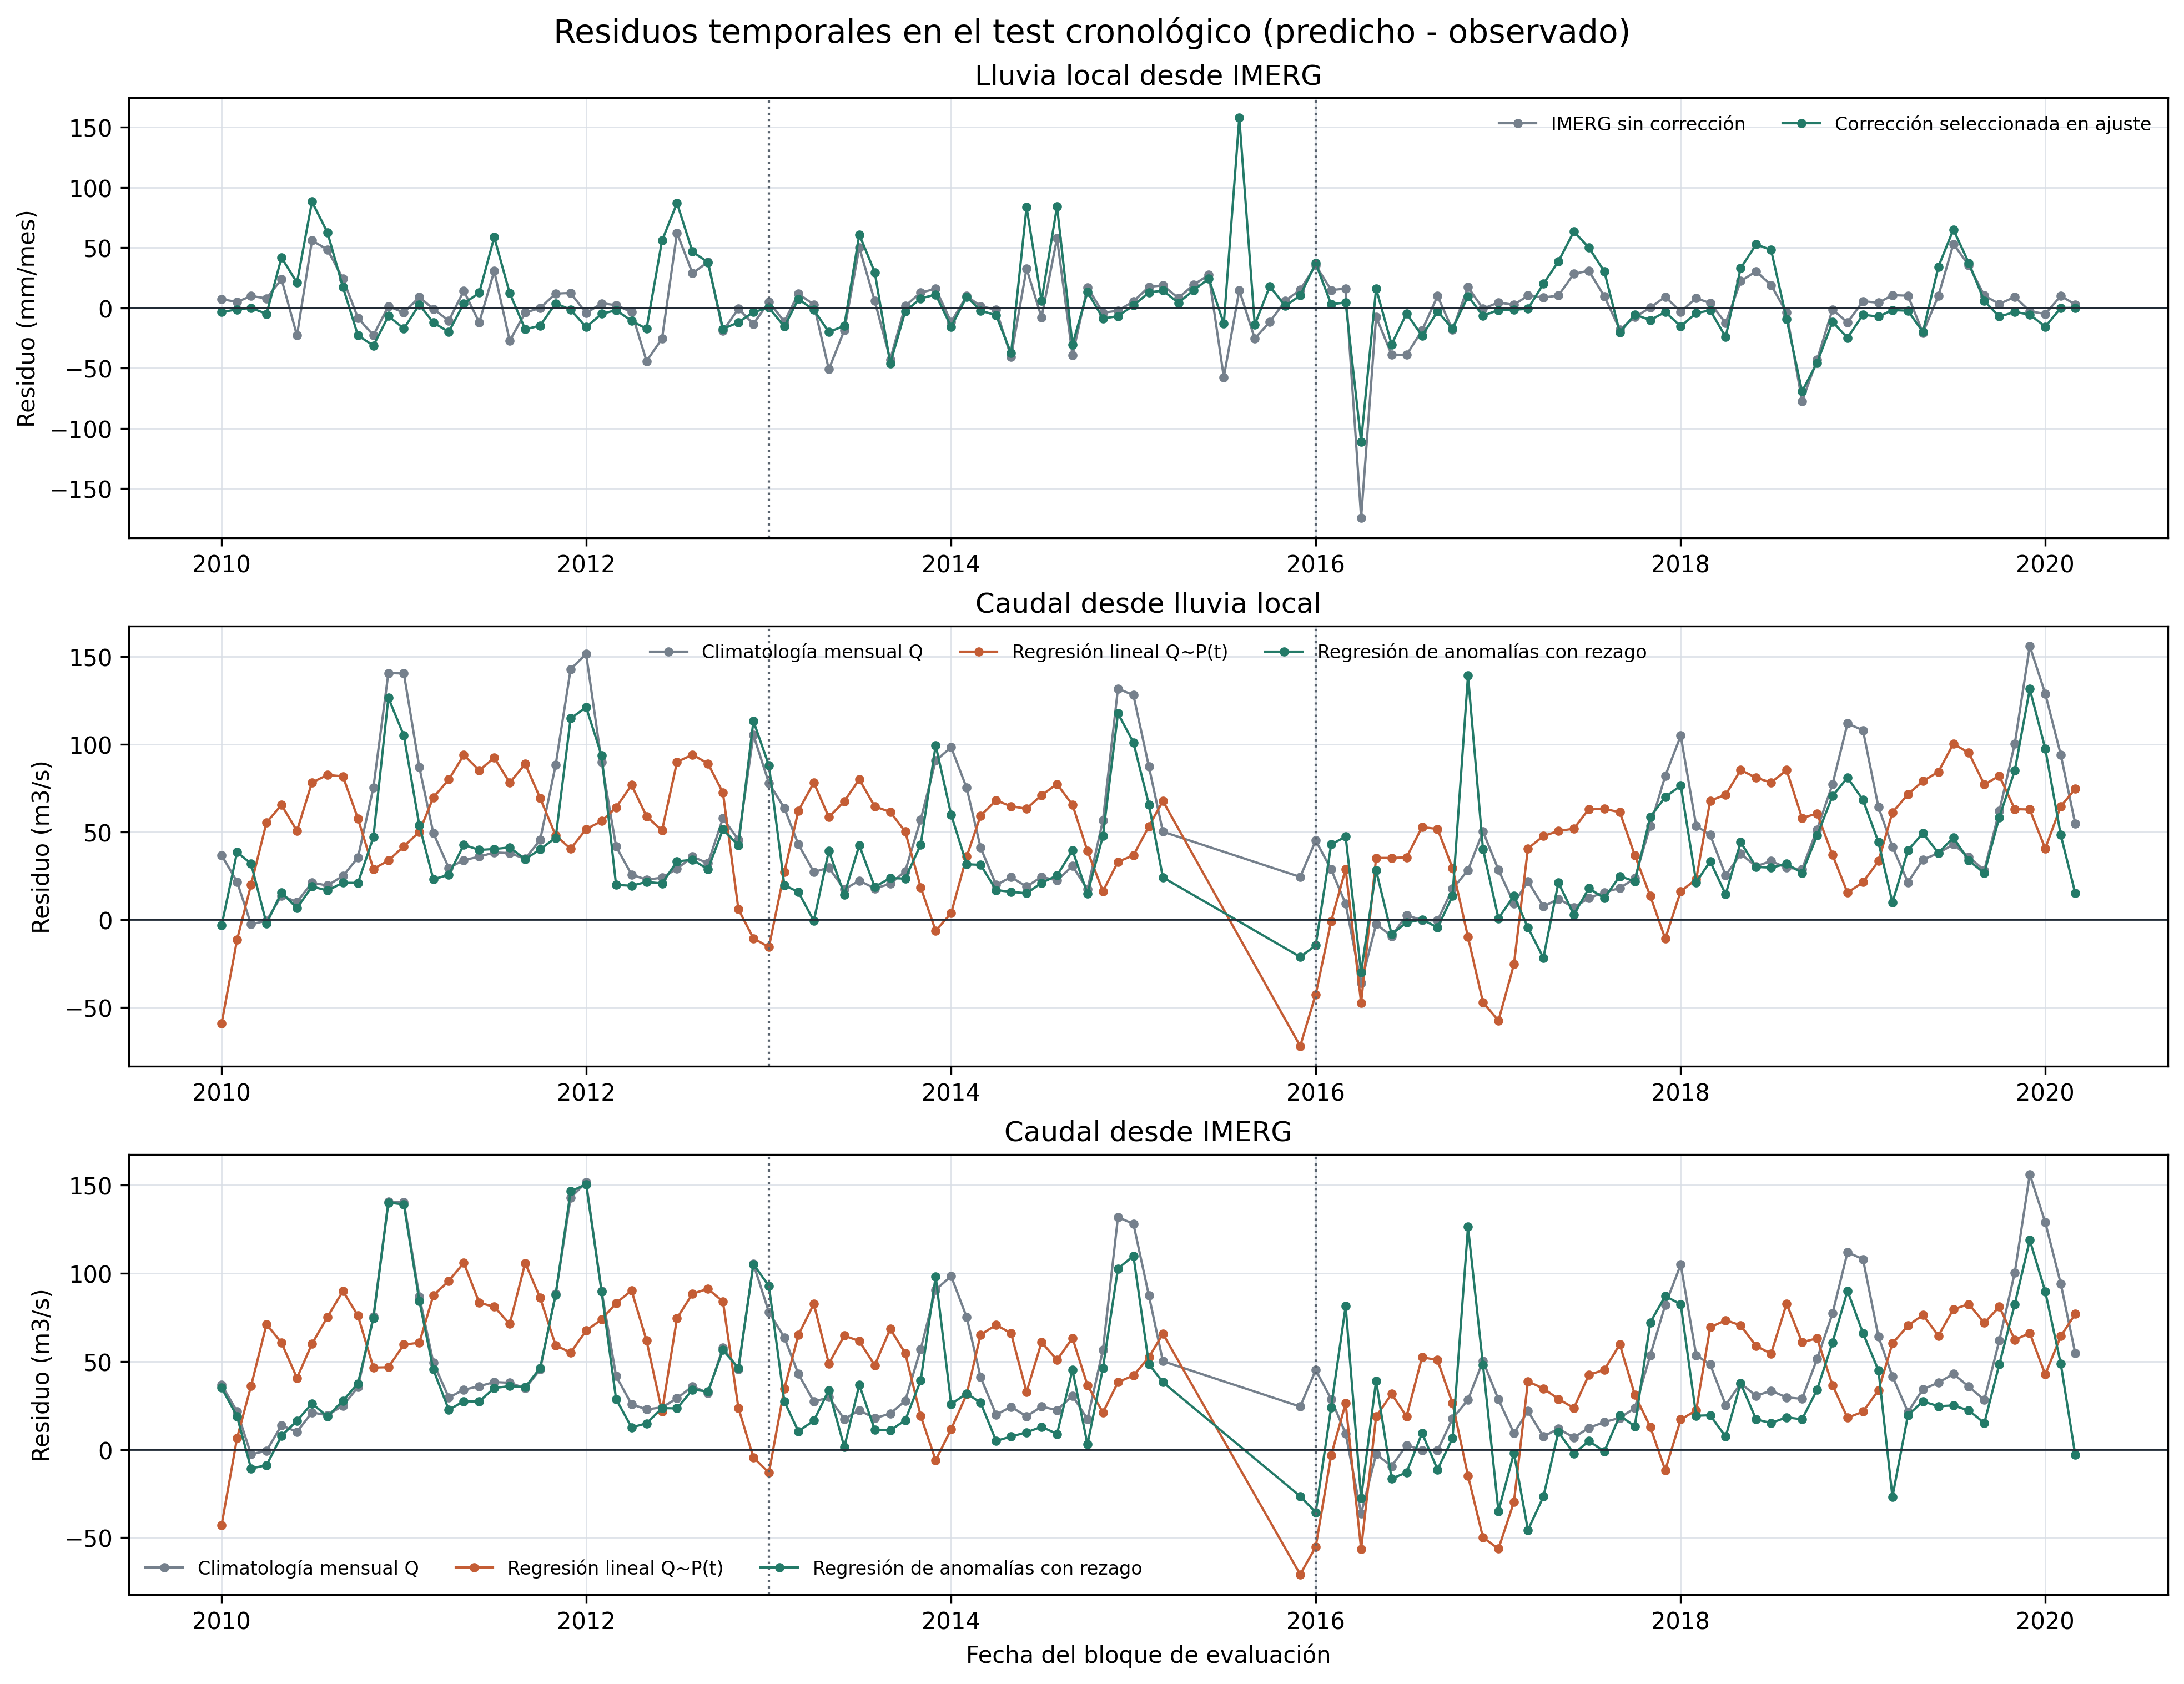
\includegraphics[width=\textwidth]{figura_2_4_residuos_en_tiempo.png}
\apanote{Residuo = predicción $-$ observado. Los picos de residuo motivaron auditorías de máximos; los datos de los bloques externos no se excluyeron.}
\end{figure}

\section{2.3. Errores, máximos y robustez temporal}
Se generaron diagnósticos temporales, por valor estimado y por mes calendario; además hay tablas por año y estación. La mejora de Q con rezago aparece en las tres ventanas, aunque los rezagos seleccionados varían (6--7 meses para $P_L$ y 7--10 para $P_I$) y el sesgo permanece positivo. El entrenamiento expansivo significa que las ventanas no son réplicas independientes. Estos resultados apoyan utilidad en las condiciones evaluadas, no generalización irrestricta ni pronóstico futuro.

\begin{table}[H]
\centering\small\singlespacing
\apatableheading{tab:maxima}{Auditoría empírica de las máximas predicciones por estrategia}
\begin{tabularx}{\textwidth}{Xlrrrr}
\toprule
Objetivo/modelo & Fecha & Predicción & Observado mismo mes & Error & Máximo observado del test \\
 & & & & \multicolumn{2}{c}{mm/mes o m$^3$/s} \\
\midrule
$P_L$ desde $P_I$, corrección log-lineal & 2015-08 & 398.42 & 240.49 & $+157.94$ & 240.49 \\
$Q$ desde $P_L$, anomalía con rezago & 2016-11 & 276.62 & 137.23 & $+139.39$ & 186.00 \\
$Q$ desde $P_I$, anomalía con rezago & 2016-11 & 263.62 & 137.23 & $+126.39$ & 186.00 \\
\bottomrule
\end{tabularx}
\apanote{Las tres máximas caen dentro del rango observado antes del test y bajo el P99 de ajuste, pero sobrepasan el máximo observado del bloque. Cada una coincide con el mayor error absoluto de su bloque. Esto indica sobreestimación de eventos concretos, no imposibilidad física ni habilidad para extremos. Fuente: \texttt{figuras/tabla\_2\_3\_maximos\_predichos.csv}.}
\end{table}

El registro B-05 documenta una primera prueba histórica de un único corte cuyo Q desde IMERG alcanzó 302.77 m$^3$/s en 2016-12. Esa estimación corresponde a un ajuste fijo hasta 2015-12 y un único rezago $k=8$; no se mezcla con la evaluación multibloque, que reajusta/selecciona cada fold y cuyo máximo fue 263.62 m$^3$/s. En la reconstrucción histórica el caudal observado simultáneo fue 170.68 m$^3$/s, por lo que la predicción sobreestimó 77.4\%. La magnitud es posible dentro del historial estacional de ajuste, pero fue deficiente para esa fecha. No constituye una prueba de crecidas ni de caudales máximos.

\section{2.4. Interpretación física, fuentes compartidas y límites}
La diferencia entre los ciclos mensuales de precipitación y caudal y la memoria estimada en rezagos es compatible con procesos de almacenamiento. En la banda 30--37$^\circ$S, el manto nival se ha relacionado con caudales de temporada cálida; estudios chilenos encuentran memoria hidrológica modulada por nieve y aguas subterráneas, y existe modelación de aportes glaciares para la cuenca del Maipo \parencite{Masiokas2006,Cortes2017,AlvarezGarreton2021,Ayala2020}. La evidencia justifica formular esa hipótesis regional, pero no atribuir el rezago predictivo seleccionado a nieve o deshielo como causa demostrada.

Rojas et al. evaluaron IMERG V06 en campañas invernales del centro-sur de Chile y encontraron errores dependientes de elevación y régimen microfísico; Alcayaga y colegas analizaron 3IMERG en estaciones de varias zonas hidroclimáticas de Chile. Esas publicaciones están más próximas al contexto local que una evaluación genérica, pero difieren del promedio mensual areal del Maipo y de su ventana temporal. da Silva et al. analiza IMERG Early, no Final; Zambrano-Bigiarini et al. examina gradientes chilenos pero no incluye IMERG. Por tanto, estos trabajos contextualizan la validación propia y no reemplazan sus 238 pares \parencite{Rojas2021,SotoAlvarez2020,DaSilva2023,Zambrano2017}.

La procedencia local se describe en el proyecto como referencia CAMELS-CL/CR2MET, y NASA especifica que IMERG Final usa información mensual de pluviómetros. Ello hace posible una dependencia entre fuentes, pero no identifica estaciones compartidas en este caso. La entrada #25 del handoff adopta V06 como versión canónica a partir de script e historial; el registro B-08 señala que no se conserva el manifiesto original de la exportación. El informe mantiene la etiqueta de proyecto V06 con esa salvedad y recomienda conservar metadatos completos en futuras descargas.

\begin{table}[H]
\centering\small\singlespacing
\apatableheading{tab:evidence}{Síntesis de resultados, interpretación y límites}
\begin{tabularx}{\textwidth}{p{2.4cm}XX}
\toprule
Resultado observado & Interpretación respaldada & Límite principal \\
\midrule
$P_I$--$P_L$: $r=.888$, sesgo $-5.50$ mm/mes & Asociación lineal alta, concordancia imperfecta; error cambia por estación/intensidad & No demuestra causa orográfica ni independencia entre fuentes \\
Lag exploratorio de anomalías cerca de 7 meses & Compatible con memoria/almacenamiento documentados regionalmente & Máximo de 13 rezagos; selección autocorrelacionada no identifica tiempo físico \\
Q con anomalía rezagada reduce MAE/RMSE en 3 folds & Evidencia retrospectiva de utilidad comparativa en las ventanas evaluadas & Entrenamiento expansivo; una familia de cuencas; no demuestra habilidad prospectiva general \\
Corrección de lluvia no mejora en agregado & Es preferible el producto sin corregir según MAE/RMSE agrupados & Desempeño puede variar por fold, evento y producto/version \\
Máximos predichos superan máximos de test & Sobreestimación de casos puntuales, dentro del rango histórico de ajuste & No es habilidad para eventos extremos ni límite físico independiente \\
\bottomrule
\end{tabularx}
\apanote{Las citas regionales respaldan plausibilidad de mecanismos, no causalidad en las series del proyecto. Los conteos, métricas y tablas provienen del CSV maestro y scripts.}
\end{table}

\section{Síntesis del punto 2}
La relación mensual IMERG--referencia muestra covariación alta pero error significativo y dependiente de magnitud. La asociación contemporánea lluvia--caudal en datos sin transformar conserva el ciclo anual; al retirar la climatología mensual se atenúa y los lags previos ofrecen señales exploratorias. En validación externa por tres bloques, la corrección para reconstruir lluvia local no supera IMERG crudo en el conjunto agregado, mientras el modelo de anomalías con rezago mejora MAE/RMSE de caudal frente a la climatología mensual y la regresión contemporánea. Persiste sesgo positivo y los rezagos varían entre folds. La conclusión más defendible es utilidad predictiva preliminar, condicionada a estos periodos, no causalidad ni generalización futura. La clasificación hidrológica de la cuenca y el balance hídrico requieren integrar los demás puntos de la tarea.

\printbibliography[title={Referencias}]

\appendix
\section{Climatología mensual usada en anomalías}
La tabla completa procede de `figuras/tabla\_2\_2\_climatologia\_referencia.csv`. Las medias, medianas y desviaciones son estadísticas entre años por mes calendario; $n$ es el número de valores válidos en la referencia 2000-06--2020-03. Las anomalías estandarizadas usan la desviación estándar muestral.

\begin{longtable}{llrrrr}
\caption{Climatología por variable y mes calendario}\label{tab:climatologyFull}\\
\toprule
Variable & Mes & $n$ & Media & Mediana & DE \\
\midrule
\endfirsthead
\toprule
Variable & Mes & $n$ & Media & Mediana & DE \\
\midrule
\endhead
\bottomrule
\endfoot
$P_L$ & Ene & 20 & 13.41 & 13.15 & 10.58 \\
$P_L$ & Feb & 20 & 12.28 & 7.54 & 11.98 \\
$P_L$ & Mar & 20 & 10.75 & 6.47 & 14.25 \\
$P_L$ & Abr & 19 & 44.40 & 27.66 & 82.02 \\
$P_L$ & May & 19 & 116.87 & 100.39 & 105.43 \\
$P_L$ & Jun & 20 & 168.08 & 132.59 & 140.73 \\
$P_L$ & Jul & 20 & 123.72 & 73.74 & 127.48 \\
$P_L$ & Ago & 20 & 118.27 & 68.83 & 108.83 \\
$P_L$ & Sep & 20 & 68.98 & 60.52 & 63.13 \\
$P_L$ & Oct & 20 & 39.75 & 21.54 & 36.29 \\
$P_L$ & Nov & 20 & 24.92 & 17.09 & 23.74 \\
$P_L$ & Dic & 20 & 13.83 & 6.37 & 17.13 \\
$P_I$ & Ene & 20 & 18.02 & 16.57 & 9.93 \\
$P_I$ & Feb & 20 & 17.49 & 15.48 & 10.36 \\
$P_I$ & Mar & 20 & 17.07 & 12.38 & 12.75 \\
$P_I$ & Abr & 19 & 37.48 & 22.82 & 44.01 \\
$P_I$ & May & 19 & 88.51 & 77.23 & 50.24 \\
$P_I$ & Jun & 20 & 140.24 & 128.37 & 72.46 \\
$P_I$ & Jul & 20 & 124.97 & 110.46 & 57.61 \\
$P_I$ & Ago & 20 & 110.88 & 107.51 & 63.02 \\
$P_I$ & Sep & 20 & 49.16 & 40.63 & 26.05 \\
$P_I$ & Oct & 20 & 35.26 & 33.56 & 23.54 \\
$P_I$ & Nov & 20 & 24.38 & 23.52 & 11.22 \\
$P_I$ & Dic & 20 & 24.55 & 23.47 & 13.64 \\
$Q$ & Ene & 20 & 177.99 & 157.16 & 98.14 \\
$Q$ & Feb & 20 & 133.96 & 117.07 & 63.75 \\
$Q$ & Mar & 20 & 93.39 & 81.55 & 34.81 \\
$Q$ & Abr & 18 & 72.55 & 70.29 & 20.59 \\
$Q$ & May & 18 & 59.15 & 60.14 & 15.03 \\
$Q$ & Jun & 19 & 60.98 & 59.83 & 18.84 \\
$Q$ & Jul & 19 & 58.92 & 55.46 & 21.05 \\
$Q$ & Ago & 19 & 61.22 & 54.03 & 23.73 \\
$Q$ & Sep & 19 & 68.88 & 63.92 & 20.71 \\
$Q$ & Oct & 19 & 95.43 & 88.36 & 33.00 \\
$Q$ & Nov & 19 & 146.08 & 121.91 & 58.97 \\
$Q$ & Dic & 20 & 192.03 & 145.66 & 100.71 \\
$R$ & Ene & 20 & 98.52 & 86.99 & 54.32 \\
$R$ & Feb & 20 & 67.42 & 59.68 & 31.68 \\
$R$ & Mar & 20 & 51.69 & 45.14 & 19.27 \\
$R$ & Abr & 18 & 38.86 & 37.65 & 11.03 \\
$R$ & May & 18 & 32.74 & 33.29 & 8.32 \\
$R$ & Jun & 19 & 32.66 & 32.05 & 10.09 \\
$R$ & Jul & 19 & 32.61 & 30.70 & 11.65 \\
$R$ & Ago & 19 & 33.88 & 29.90 & 13.13 \\
$R$ & Sep & 19 & 36.90 & 34.24 & 11.09 \\
$R$ & Oct & 19 & 52.82 & 48.91 & 18.27 \\
$R$ & Nov & 19 & 78.25 & 65.30 & 31.59 \\
$R$ & Dic & 20 & 106.29 & 80.62 & 55.74 \\
$T$ & Ene & 20 & 8.28 & 8.43 & 1.21 \\
$T$ & Feb & 20 & 8.47 & 8.54 & 1.23 \\
$T$ & Mar & 20 & 6.88 & 6.68 & 1.46 \\
$T$ & Abr & 19 & 1.83 & 1.63 & 2.32 \\
$T$ & May & 19 & $-4.30$ & $-5.00$ & 2.50 \\
$T$ & Jun & 20 & $-7.78$ & $-8.02$ & 1.50 \\
$T$ & Jul & 20 & $-8.44$ & $-8.18$ & 1.46 \\
$T$ & Ago & 20 & $-7.30$ & $-6.94$ & 1.43 \\
$T$ & Sep & 20 & $-5.71$ & $-5.80$ & 1.51 \\
$T$ & Oct & 20 & $-2.89$ & $-2.74$ & 1.19 \\
$T$ & Nov & 20 & 0.26 & 0.31 & 1.15 \\
$T$ & Dic & 20 & 4.41 & 4.25 & 1.76 \\
\end{longtable}
\apanote{Unidades: $P_L$, $P_I$, $R$ en mm/mes; $Q$ en m$^3$/s; $T$ en $^\circ$C; DE = desviación estándar muestral. La lámina $R$ deriva de $Q$ y no se interpreta como observación independiente.}

\section{Archivos reproducibles asociados}
\begin{itemize}
\item Relaciones: \texttt{scripts/04\_analisis\_precipitacion.py}; tablas \texttt{tabla\_2\_1\_*}; Figura~\ref{fig:scatter}.
\item Anomalías/rezagos: \texttt{scripts/05\_anomalias\_rezagos.py}; tablas \texttt{tabla\_2\_2\_*}; Figura~\ref{fig:lags}.
\item Modelos multibloque: \texttt{scripts/06\_modelos\_validacion\_temporal.py}; archivos \texttt{tabla\_2\_3\_metricas\_fuera\_ajuste.csv}, \texttt{tabla\_2\_3\_metricas\_por\_bloque.csv}, \texttt{tabla\_2\_3\_seleccion\_modelos\_ajuste.csv}, \texttt{tabla\_2\_3\_maximos\_predichos.csv}, predicciones y desgloses anuales/mensuales/estacionales; Figuras~\ref{fig:validation} y \ref{fig:residuals}.
\item Entrada única para cálculos: \texttt{datos/datos\_mensuales\_maipo.csv}.
\end{itemize}

\end{document}